\documentclass[twoside,11pt]{article}\usepackage{amsmath,amsfonts,amsthm,fullpage}
\usepackage{amsmath}
\usepackage{amssymb}
\usepackage{listings}
\setlength{\parindent}{0pt}
\usepackage{graphicx}
\usepackage{bm}
% Use the standard article template.
%
% The geometry package allows for easy page formatting.
\usepackage{geometry}
\geometry{letterpaper}
% Load up special logo commands.
\usepackage{doc}
% Package for formatting URLs.
\usepackage{url}
% Packages and definitions for graphics files.
\usepackage{epstopdf}
\DeclareGraphicsRule{.tif}{png}{.png}{`convert #1 `dirname #1`/`basename #1 .tif`.png}

\def\argmin{\operatornamewithlimits{arg\, min}}
\newcommand{\rbr}[1]{\left(#1\right)}
\newcommand{\cbr}[1]{\left\{#1\right\}}
\newcommand{\Ncal}{\mathcal{N}}

%
% Set the title, author, and date.
%
\title{Parallel Processing using MPI - Get Genetic Sequence Motifs - Using Hamming Distance}
\author{Ajay D'Souza }
\date{}

\begin{document}


\maketitle



% Add an abstract.
\begin{abstract}
Implement a version of a Master Slave Parallel Algorithm for a Motif Finding Problem for a set of sequences
\end{abstract}

% Add various lists on new pages.
\pagebreak
\tableofcontents

\pagebreak
\listoffigures


% Start the paper on a new page.
\pagebreak

%
% Body text.
%
\section{Algorithm Description}
\label{algorithm}
\begin{enumerate}
\item
We perform a bounded depth first binary tree exploration on the string of bits to explore the possible $\sum_{c=0}^{d} 2^c *{l\choose c} * n$  , i.e.,  $\mathcal{O}(n* 2^d * {l\choose d})$ possible combination. The search is bounded by the max hamming distance d.
\item
The bit string fo the first number in the input list is picked and its bit positions are flipped one position at a time as the tree is explored. This exploration is one till
 hamming distance up to $d$ is reached between this flipped bit string and the original first number 
\item
A stack data structure (std::vector) is used for the depth first search. Depth first search also ensures that the worker processors get numbers for exploring as soon as possible
\item
Each entry in the stack is a string with bits explored up to a point the position of which is also stored along with the string
\item
When a element is popped from the stack, a bit string along with the information of the position till which it has been explored from its MSB is available for further exploration.
\item
If hamming distance of a bit string is $\le d$ for the first number, then check if hamming distance of any of the other numbers is $>d$. If hamming distance for all is $\le d$ save the bit string in results
\item
If the hamming distance of $>d$ is reached between a bit string sequence and the first number, then that particular bit string sequence need not be explored further
\item
Similarly if hamming distance of $>d$ is reached between a bit string sequence and the any number only in the part of the bit string that has been explored so far then that string sequence need not be explored further
\item
If a string has not reached its end and has to be explored further then push a copy of the string to the stack with the next bit flipped and bit position incremented, similarly push the copy of the same string to the stack with no change but with the bit position incremented
\end{enumerate}

\subsection{Hamming Distance}
The hamming distance between two numbers of same byre length is got by counting the $1's$ from the result of the exclusive or bit operation on them 


\section{Protocol Used}
\label{protocol_used}
The communication protocol used for the parallel master slave algorithm is shown in figure $\eqref{Communication Protocol}$. The following is a outline of the steps of the communication protocol
\begin{enumerate}
\item
The Master processor will read the data files and then send n,l,d,master depth and the input array of size n to each the worker processors using multiple $\verb|MPI_Send|$ 5 calls
\item
Each of the worker processors will receive the  n,l,d,\verb|master_depth| and the input array of size n data sent by the master using the same number of $\verb|MPI_Recv|$ 5 calls
\item
On receiving all the n,l,d,master depth and input data each worker processor will execute a $\verb|MPI_Recv|$ with $\verb|MPI_ANY_TAG|$ in a loop to receive further data from the master
\item
The Master after it has sent the n,l,d,master depth and input data to each of the processor, will then do its partial exploration of the first number in input, to a depth of \verb|master_depth| using depth first search as described above. Any bit strings which meet the hamming distance of $\le d$ for all numbers will be added to results.
\item
Once the \verb|master_depth| is reached in the master, the bit string is sent to the worker process on a round robin basis using \verb|MPI_Send|. This ensures uniform distribution of numbers between the worker processors
\item
Once the master has completed exploring the bit string tree to a depth of \verb|master_depth| and completed sending the numbers to the worker process, it will then send a message to each of the worker processes using \verb|MPI_Send| using the custom tag \verb|MPI_TAG_MASTER_NO_NUMS_TO_SEND| indicating it has no more numbers to send to them
\item
If worker processors which are in a loop with \verb|MPI_RECV with MPI_ANY_TAG| from the master, receive a number to explore (TAG=0), the worker process will explore that number and send any results back to the master using \verb|MPI_Send|, the worker then continues in the loop with \verb|MPI_RECV| with \verb|MPI_ANY_TAG| from the source as master. If the worker process receives a \verb|MPI_TAG_MASTER_NO_NUMS_TO_SEND| tag from the master then it will break this loop. It will then send a \verb|MPI_Send| message to the master with tag \verb|MPI_worker_TERMINATING| and terminate
\item
After the master has sent the \verb|MPI_TAG_MASTER_NO_NUMS_TO_SEND| tag to the worker processors earlier, the Master Processors will be in a loop with a \verb|MPI_Recv| with \verb|MPI_ANY_SOURCE| and \verb|MPI_ANY_TAG| to get results $(tag=0)$ or termination information (\verb|MPI_worker_TERMINATING|) from the worker processors. If the master received results $(tag=0)$ it will add the results to its result list, if the master gets a termination tag (\verb|MPI_worker_TERMINATING|) from the worker it will increment its counter of the number of workers that have terminated. When this count of the number of worker processors terminated equals $p-1$ where $p$ is the total number of processors the master will break the loop and terminate
\item
This protocol ensures that worker process overlaps its computation with communication. When it has received a number the worker processor will only spend time on computation and will not waste cycles on a blocking \verb|MPI_Recv| on the master. Only once it computation is done and it has sent any results to the master using \verb|MPI_Send| will the worker go and block with \verb|MPI_Recv| till it received a number or a no more number message from the master. Since MPI ensures that the The messages sent from the master are left on the queue till the worker process receives them off the queue, the worker will never be held back in a blocking state when it has pending computation of a number it has received.
\end{enumerate}




\begin{figure}[!htbp]
\centering
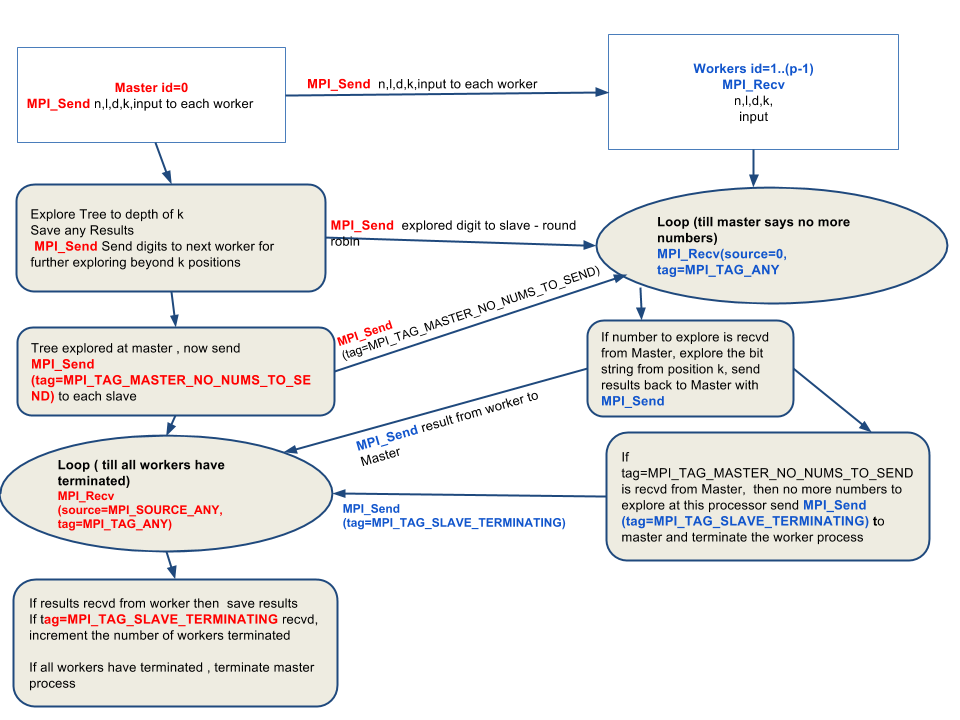
\includegraphics[scale=.46]{images/prog1_communication_protocol} 
\caption{Communication Protocol}
\label{Communication Protocol}
\end{figure}


\pagebreak
\section{Runtime Performance and Plots}
The algorithm was executed for the following parameters
\begin{itemize}
\item
size n = 200,300,400,500,600
\item
master depth to explore k = 4,10,14
\item
Number of parallel processors p=1,4,8,12,16,24
\item
Hamming distance d=15,16,17
\item
Bit string length l = 30,33,34,35,36
\end{itemize}
The run time for the algorithm increases as l,d and n are increased as this increases the search space. By varying k we can determine the sharing of the load between the master and the worker processes. Increasing k will increase the computation on the master and reduce that on the workers in the worst case and reducing k will be vice versa. So choosing the right value of $k$ for distribution of load between processors for optimum efficiency is important. While increasing the number of processors improves performance, a optimum value of $k$ in the range of $10-12$ gives the best improvement in performance as p was increased to $24$. 

\subsection{Runtime Performance for Serial Algorithm P=1}
 The run time in the serial algorithm for the worst case is of the order of 
\begin{align}
T(n,1)&= \sum_{c=0}^{d} 2^c *{l\choose c} * n\nonumber\\
&=\mathcal{O}( 2^d * {l\choose d} * n ) \label{p1_runtime}
\end{align} 
The following is the performance plot for the serial algorithm with p=1. The hamming distance d and the length of the bit string where fixed and the size of number n was increased. The following is the plot of the runtime in seconds for different values of n. As can be seen from plot $\eqref{Serial Runtime Vs N for p=1 l=30 d=15}$ the serial algorithm runtime increases linearly with n as expected from $\eqref{p1_runtime}$. However the runtime for the serial algorithm increases asymptotically with the length of the integer l which is  as expected from $\eqref{p1_runtime}$. The increase in runtime with $l$ can be seen in plot $\eqref{Serial Runtime Vs N for p=1 l=30 d=15}$

\begin{figure}[!htbp]
\centering
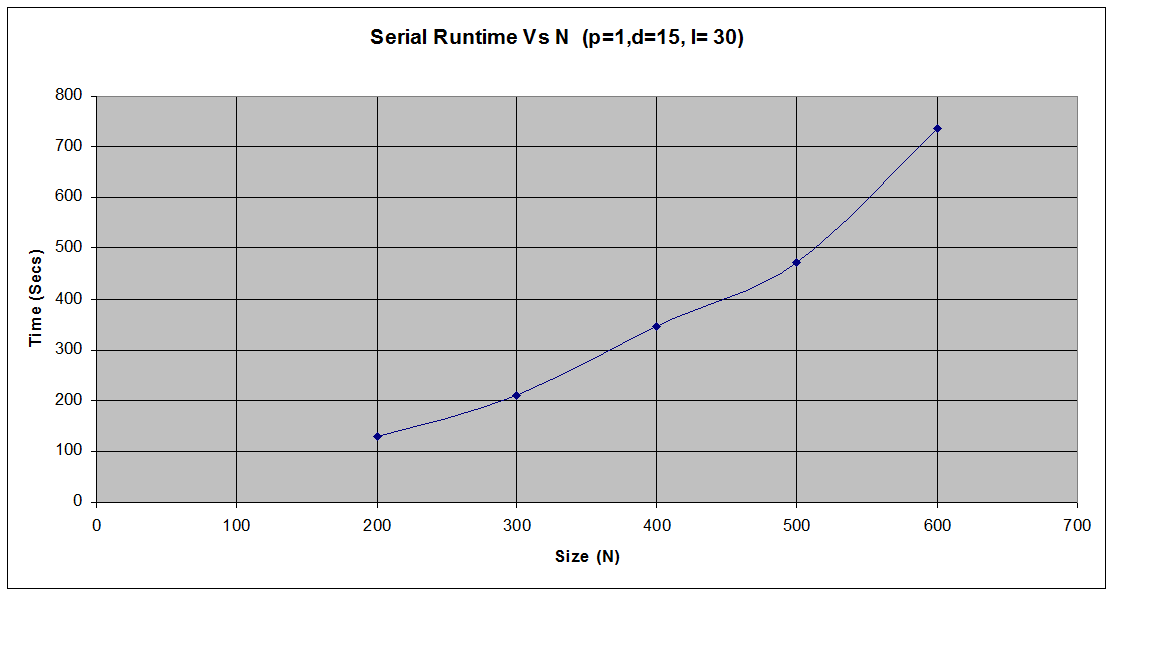
\includegraphics[scale=.46]{images/p1-l=30-d=15} 
\caption{Serial Runtime Vs N for p=1 l=30 d=15}
\label{Serial Runtime Vs N for p=1 l=30 d=15}
\end{figure}

\begin{figure}[!htbp]
\centering
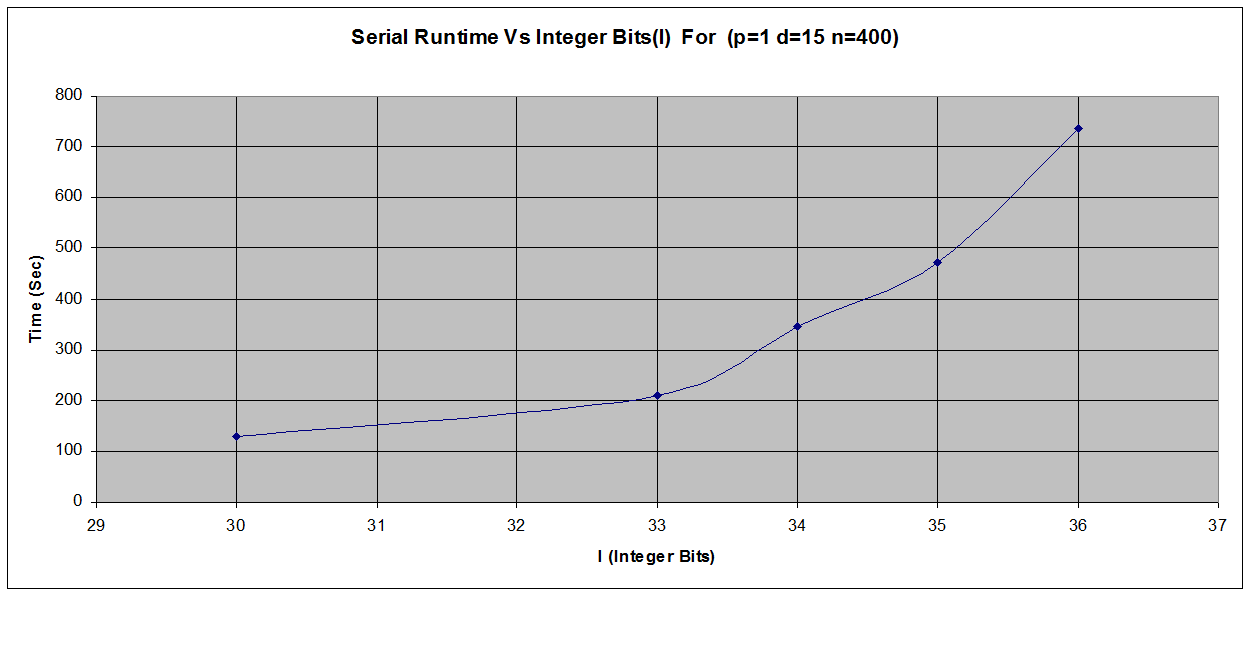
\includegraphics[scale=.46]{images/p1-vl-d=15} 
\caption{Serial Runtime Vs L for p=1 d=15 n=400}
\label{Serial Runtime Vs L for p=1 d=15 n=400}
\end{figure}




\pagebreak
\subsection{Runtime Performance - Plot of Master Depth K Vs Runtime for varying No of Processors P}
The following is the performance plot of Runtime Vs k the Master Depth for different values of P the number of processors while keeping N,l and d fixed. $k$ determines the distribution of work between the master and worker processors as $\mathcal{O}(2^k)$ digits are to be distributed to the worker processors for exploring. So a right value of $k$ determines the optimum division of work between the master and workers for the best efficiency and runtime.

As can be seen from the plots for the parameters considered, a value of around $k=10$ gives the best improvement in runtime even across different numbers of processors and for the different values of $n,l,d$ considered. A depth of $k=10$ will in the worst case generate $2^10$ problems to be distributed among the $p-1$ worker processors. While increasing the number of processors from $4$ to $24$ does improve the runtime for the processors considered.

The parallel runtime for the algorithm with the correct value of  k in the range, $10<k<12$ and for number of processors $p=24$ is almost 6 times faster than the serial run time of the algorithm for the same size of the problem. For e.g for $l=36,n=400$ the serial algorithm has a runtime of $750$ seconds, the parallel algorithm with $p=24$, $k=11$ in comparison has a run time of $150$ seconds for the same problem size. The speedup of the parallel algorithm with the right $p$ and $k$ widens over the runtime of the serial algorithm as the size of the problem as defined by the Integer length $l$ increases.

The following are the plots K Vs Runtime for varying No of Processors for various n,l,d values of 
\begin{enumerate}
\item
n=200 l=30 d=17 $\eqref{K Vs P for n=200 l=30 d=17}$
\item
n=300 l=33 d=15 $\eqref{K Vs P for n=300 l=33 d=15}$
\item
n=400 l=34 d=15 $\eqref{K Vs P for n=400 l=34 d=15}$
\item
n=500 l=35 d=15 $\eqref{K Vs P for n=500 l=35 d=15}$
\item
n=600 l=36 d=16 $\eqref{K Vs P for n=600 l=36 d=16}$
\end{enumerate}

\begin{figure}[!htbp]
\centering
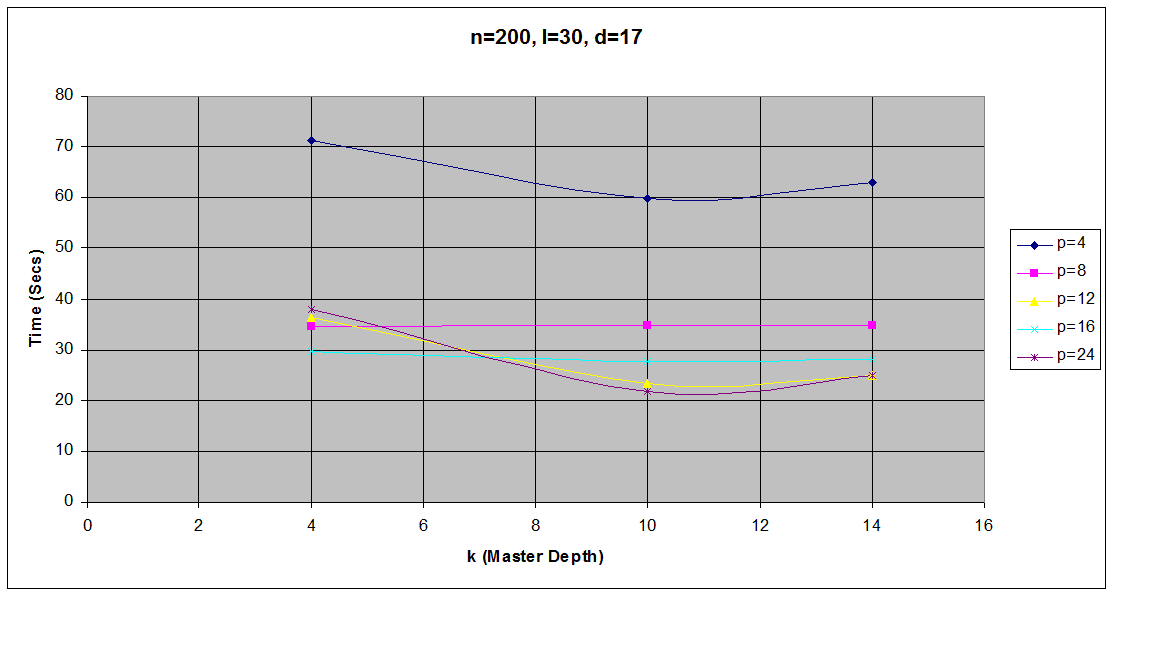
\includegraphics[scale=.46]{images/nld_n=200-l=30-d=17} 
\caption{Runtime Vs K/P for n=200 l=30 d=17}
\label{K Vs P for n=200 l=30 d=17}
\end{figure}

\begin{figure}[!htbp]
\centering
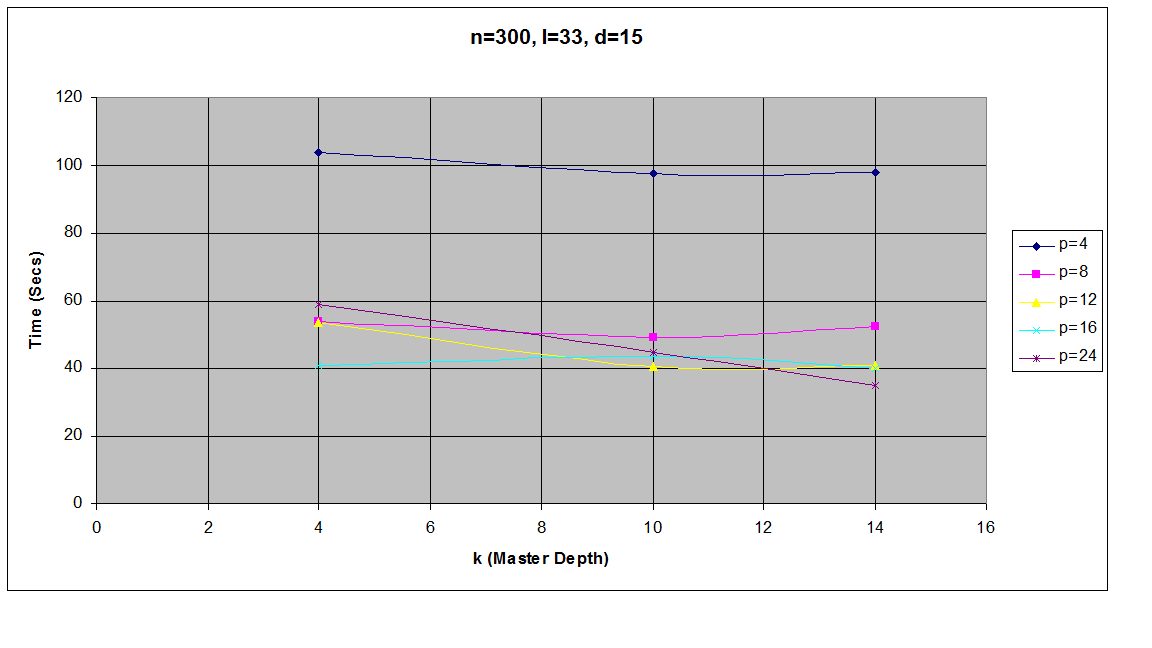
\includegraphics[scale=.46]{images/nld_n=300-l=33-d=15} 
\caption{Runtime Vs K/P for n=300 l=33 d=15}
\label{K Vs P for n=300 l=33 d=15}
\end{figure}

\begin{figure}[!htbp]
\centering
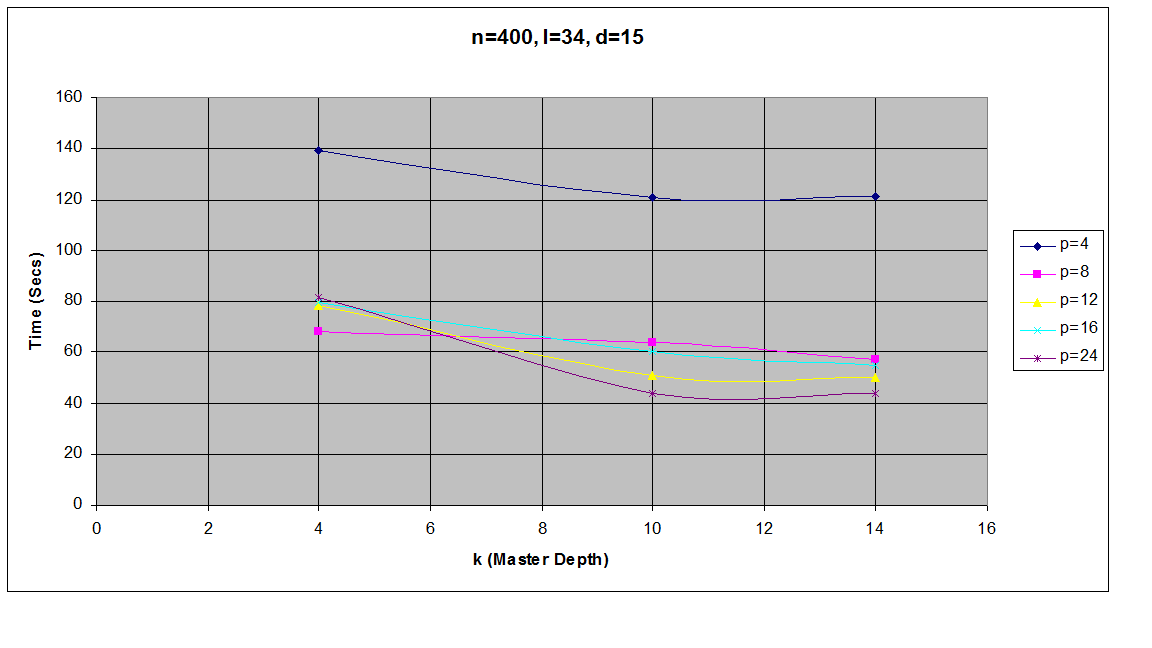
\includegraphics[scale=.46]{images/nld_n=400-l=34-d=15} 
\caption{Runtime Vs K/P for n=400 l=34 d=15}
\label{K Vs P for n=400 l=34 d=15}
\end{figure}

\begin{figure}[!htbp]
\centering
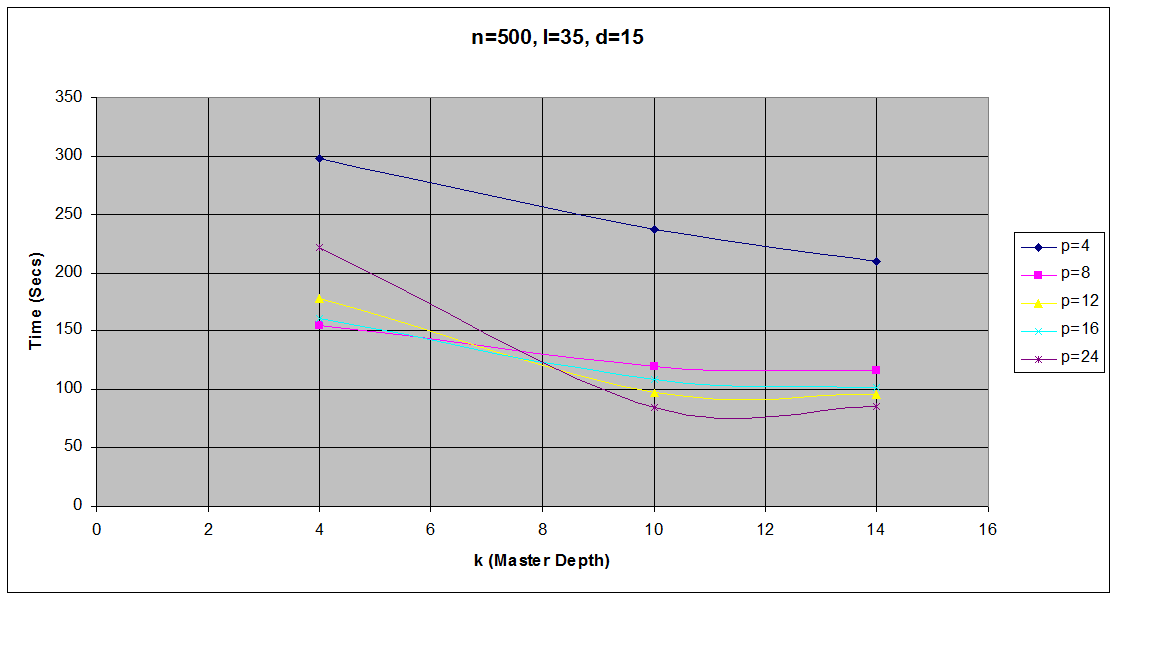
\includegraphics[scale=.46]{images/nld_n=500-l=35-d=15} 
\caption{Runtime Vs K/P for n=500 l=35 d=15}
\label{K Vs P for n=500 l=35 d=15}
\end{figure}

\begin{figure}[!htbp]
\centering
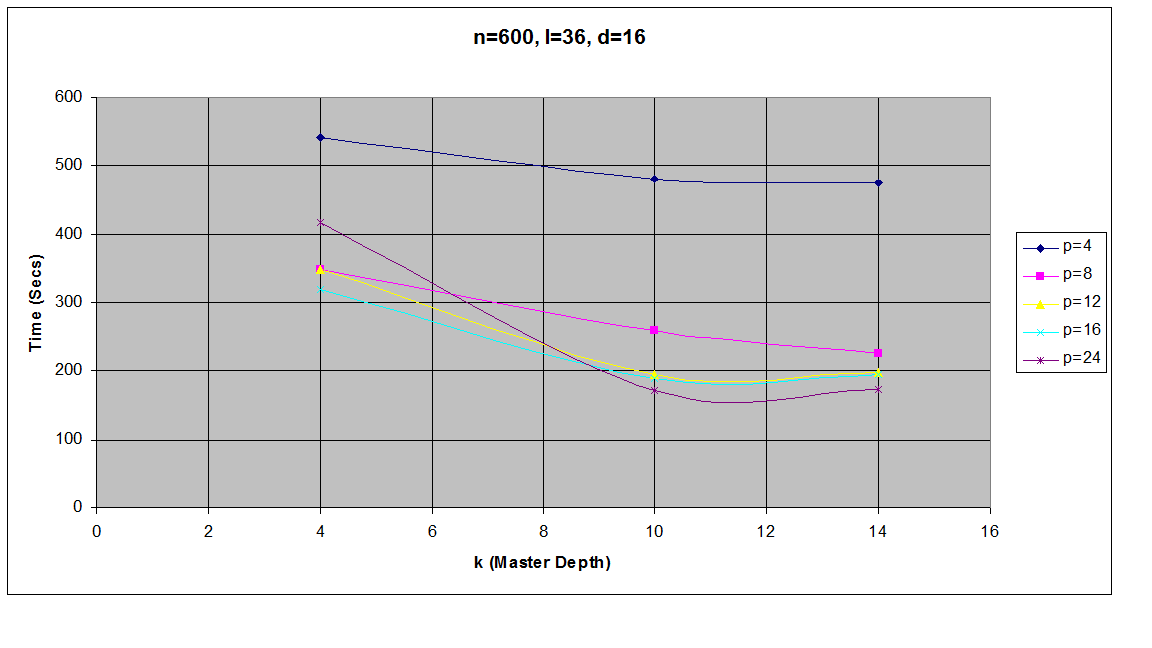
\includegraphics[scale=.46]{images/nld_n=600-l=36-d=16} 
\caption{Runtime Vs K/P for n=600 l=36 d=16}
\label{K Vs P for n=600 l=36 d=16}
\end{figure}





\pagebreak
\subsection{Runtime Performance - Plot of N Vs Runtime for varying No of Processors P}

The following are the plots of N Vs Runtime for varying No of Processors for various k,l,d values of 
\begin{enumerate}
\item
k=4 l=30 d=17 $\eqref{N Vs P for k=4 l=30 d=17}$
\item
k=10 l=30 d=17 $\eqref{N Vs P for k=10 l=30 d=17}$
\item
k=14 l=30 d=17 $\eqref{N Vs P for k=14 l=30 d=17}$
\end{enumerate}
As can be seen runtime increase is linear with respect to $N$. The runtime decreases when the number of processors are increased. However greater divergence in runtime across the values of number processors used p, can be seen as $N$ increases. From the three plots for values of $k$ of $4,10,14$, runtime increases as $k$ is increased. This is more noticeable as the number of processors $p$ is increased and $N$ is at higher values. For eg. the runtime for $k=10$ for number of processors $p=24$ for $N=500$ is almost half of the runtime for $k=4$. Thus for a given number of processors better efficiencies are achieved at the correct value of $k$ 

\begin{figure}[!htbp]
\centering
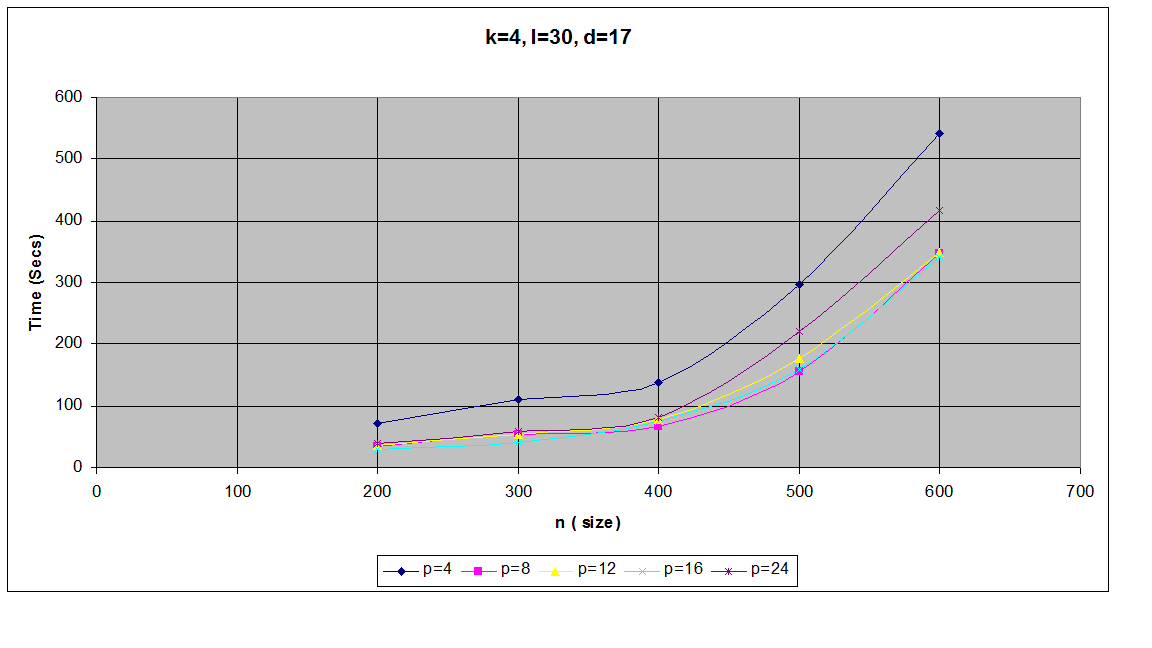
\includegraphics[scale=.46]{images/kld_k=4-l=30-d=17} 
\caption{Runtime Vs N/P for k=4 l=30 d=17}
\label{N Vs P for k=4 l=30 d=17}
\end{figure}

\begin{figure}[!htbp]
\centering
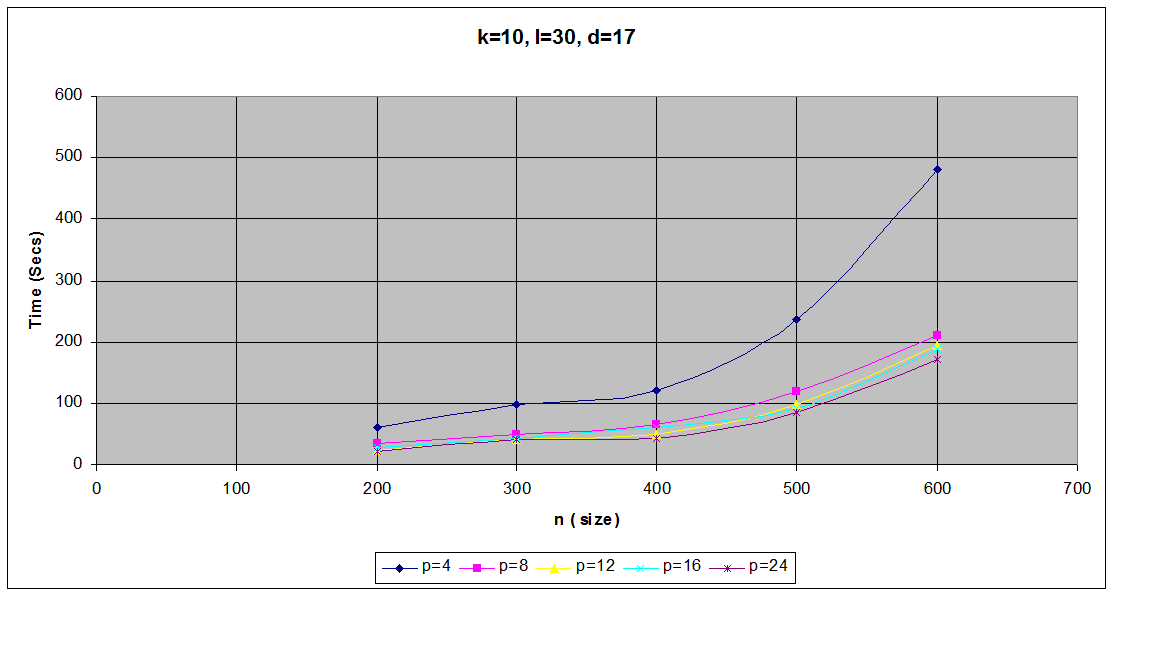
\includegraphics[scale=.46]{images/kld_k=10-l=30-d=17} 
\caption{Runtime Vs N/P for k=10 l=30 d=17}
\label{N Vs P for k=10 l=30 d=17}
\end{figure}


\begin{figure}[!htbp]
\centering
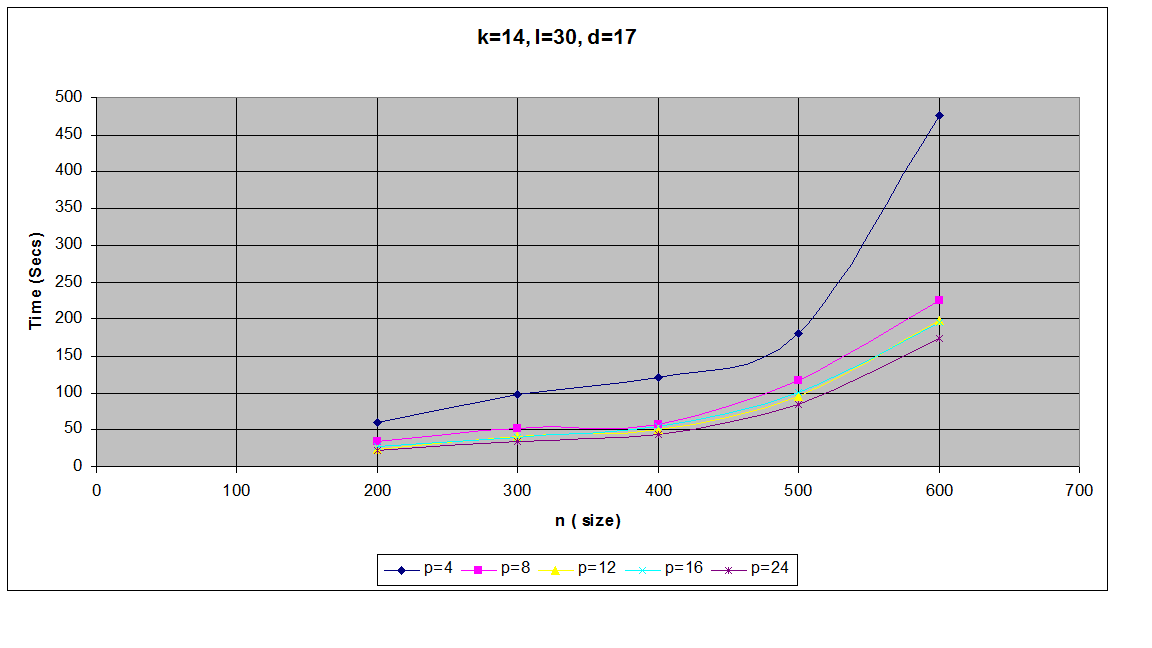
\includegraphics[scale=.46]{images/kld_k=14-l=30-d=17} 
\caption{Runtime Vs N/P for k=14 l=30 d=17}
\label{N Vs P for k=14 l=30 d=17}
\end{figure}




\pagebreak
\subsection{Runtime Performance - Plot of Master Depth K Vs Runtime for various sizes of N}

The following are the plots the Master Depth K Vs Runtime for sizes of $N={200,300,400,500,600}$ for various p,l,d values of 
\begin{enumerate}
\item
p=4 l=30 d=17 $\eqref{K Vs N for p=4 l=30 d=17}$
\item
p=8 l=30 d=17 $\eqref{K Vs N for p=8 l=30 d=17}$
\item
p=12 l=30 d=17 $\eqref{K Vs N for p=12 l=30 d=17}$
\item
p=16 l=30 d=17 $\eqref{K Vs N for p=16 l=30 d=17}$
\item
p=24 l=30 d=17 $\eqref{K Vs N for p=24 l=30 d=17}$
\end{enumerate}
From the plots it an be seen that while the runtime increases with $N$, it does so linearly. As discussed earlier as $P$ is increased from $4$ to $24$ the runtime characteristics of $K$ are more pronounced. Around $K=10$ almost appears to be a inflexion point in the curve in terms of runtime. However compared to $p=4$ at $p=24$, the curve seems to show a pronounced inflexion at $k=10$ with a drop in runtime by over half when compared with $k=4$. It can also be seen by comparing the plots for $p=4$ and $p=24$ that for $k=4$ and $n=600$ the Runtimes are essentially the same, where as at $k=10$ the same plot shows the runtime dropping to half between $p=4$ and $p=24$. This shows that increasing the number of processors by itself will not give a improvement in performance, we need to have the right value of $k$ to ensure that the processors are put to optimum use for the best efficiency and runtime.

\begin{figure}[!htbp]
\centering
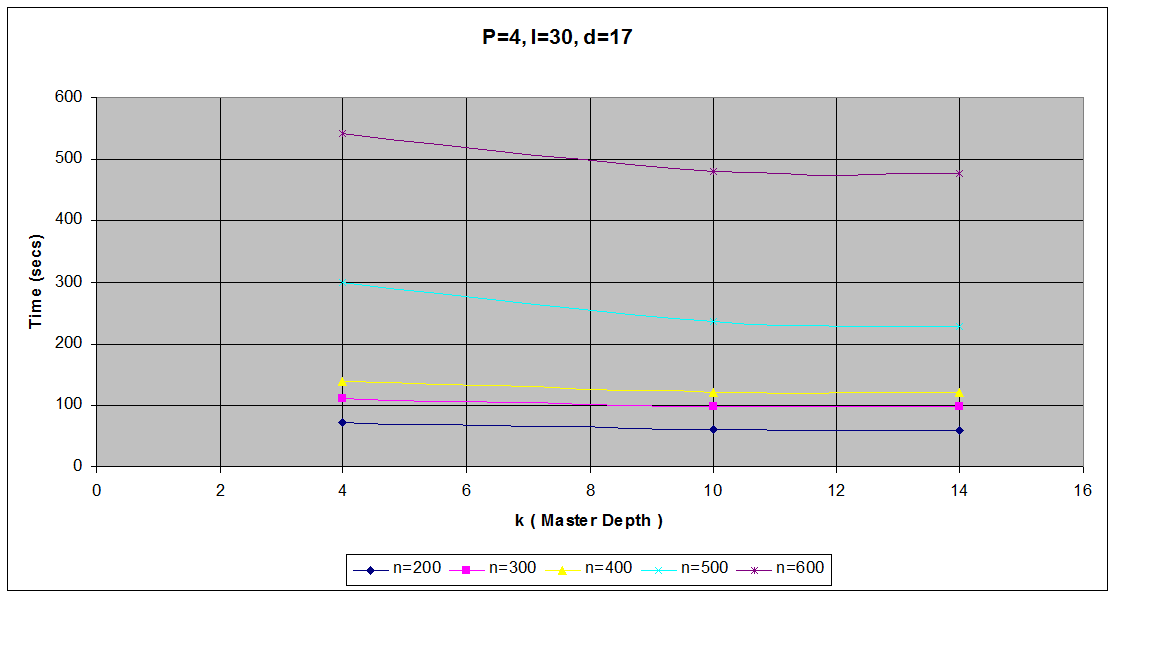
\includegraphics[scale=.46]{images/pld_p=4-l=30-d=17} 
\caption{Runtime Vs K/N for p=4 l=30 d=17}
\label{K Vs N for p=4 l=30 d=17}
\end{figure}

\begin{figure}[!htbp]
\centering
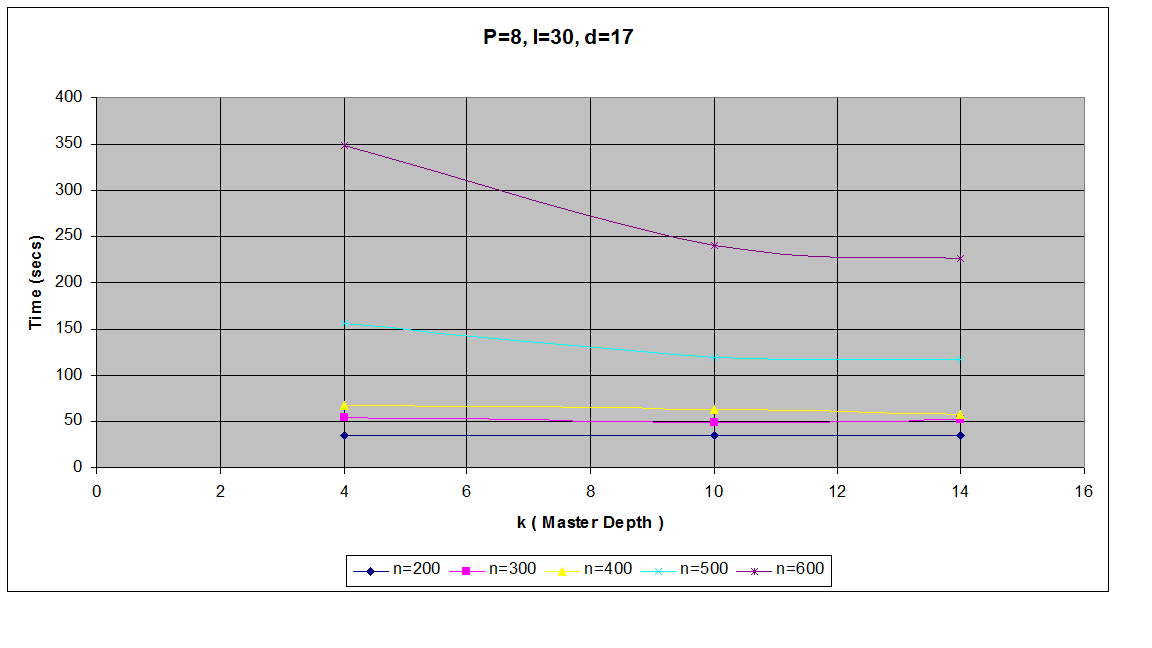
\includegraphics[scale=.46]{images/pld_p=8-l=30-d=17} 
\caption{Runtime Vs K/N for p=8 l=30 d=17}
\label{K Vs N for p=8 l=30 d=17}
\end{figure}

\begin{figure}[!htbp]
\centering
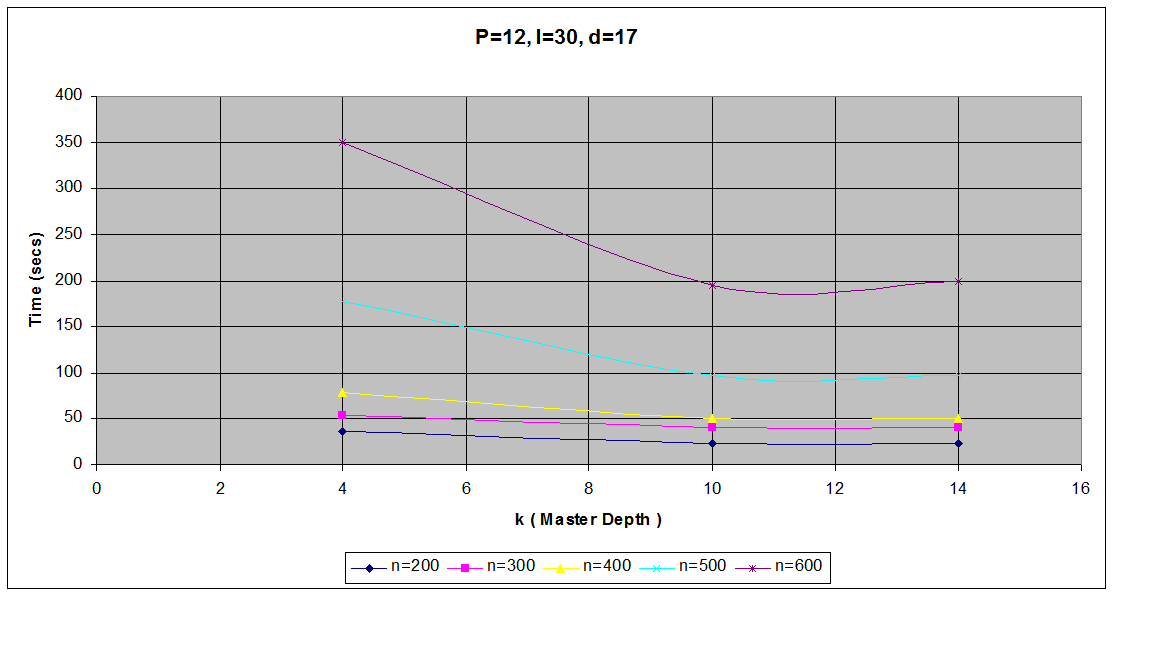
\includegraphics[scale=.46]{images/pld_p=12-l=30-d=17} 
\caption{Runtime Vs K/N for p=12 l=30 d=17}
\label{K Vs N for p=12 l=30 d=17}
\end{figure}

\begin{figure}[!htbp]
\centering
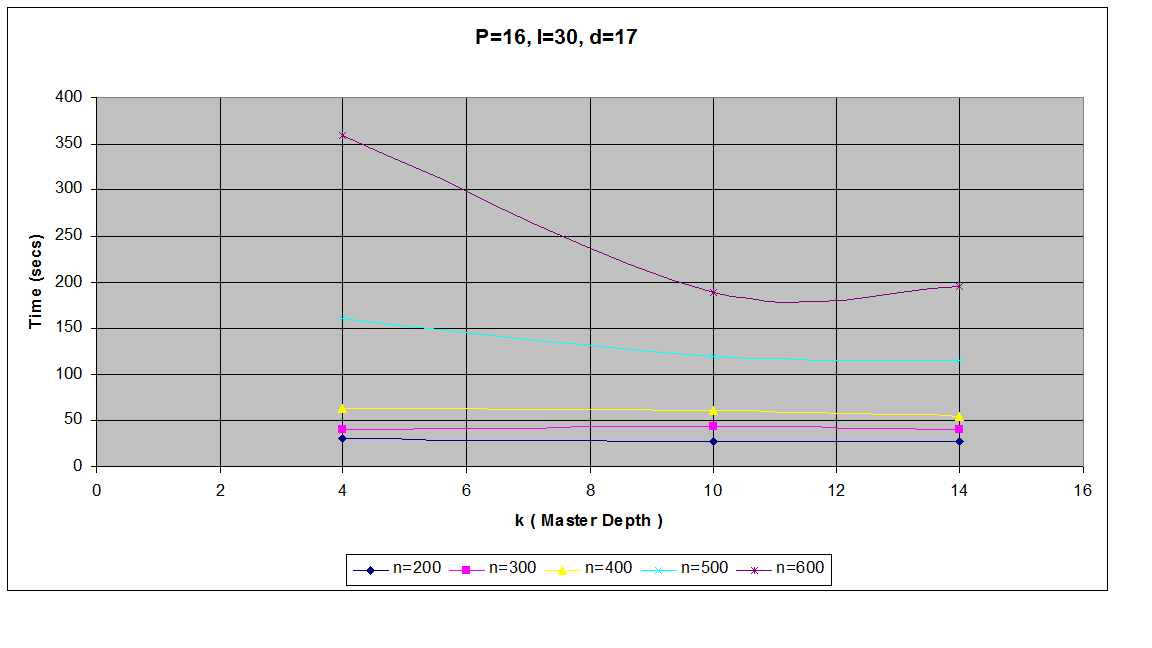
\includegraphics[scale=.46]{images/pld_p=16-l=30-d=17} 
\caption{Runtime Vs K/N for p=16 l=30 d=17}
\label{K Vs N for p=16 l=30 d=17}
\end{figure}

\begin{figure}[!htbp]
\centering
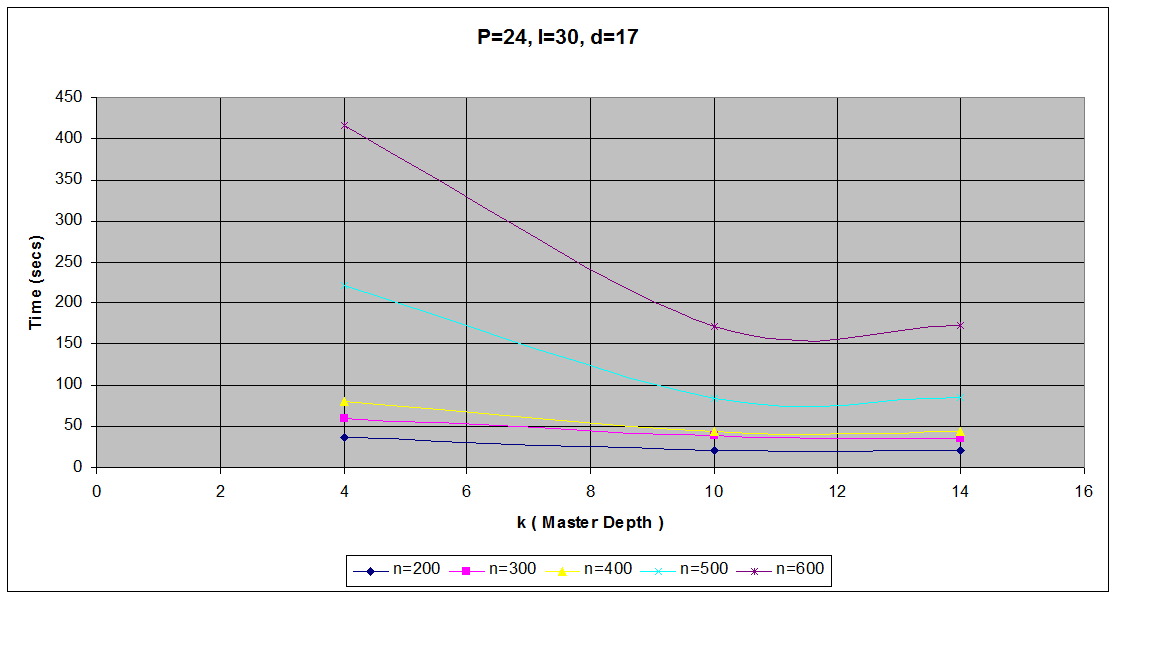
\includegraphics[scale=.46]{images/pld_p=24-l=30-d=17} 
\caption{Runtime Vs K/N for p=24 l=30 d=17}
\label{K Vs N for p=24 l=30 d=17}
\end{figure}




\pagebreak
\subsection{Runtime Performance - Plot of Master Depth K Vs Runtime for various Integer Lengths of L}

The following are the plots the Master Depth K Vs Runtime for Integer Lengths of $L={30,33,34,35,36}$ for various p,d,n values of 
\begin{enumerate}
\item
p=4 d=15 n=400 $\eqref{Runtime Vs K/L for p=4 d=15 n=400}$
\item
p=8 d=15 n=400 $\eqref{Runtime Vs K/L for p=8 d=15 n=400}$
\item
p=12 d=15 n=400 $\eqref{Runtime Vs K/L for p=12 d=15 n=400}$
\item
p=16 d=15 n=400 $\eqref{Runtime Vs K/L for p=16 d=15 n=400}$
\item
p=24 d=15 n=400 $\eqref{Runtime Vs K/L for p=24 d=15 n=400}$
\end{enumerate}
From the plots it an be seen that the runtime increases substantially with even small increases in $L$, far more than the linear increase seen with $N$ in the earlier plots. The same conclusions as earlier can be drawn with respect to $p$ and $k$. There seems to be a inflexion point in $k$ in the range of $k=10-12$. From $k=4$ to this inflexion we can see a sharp improvement in runtime, further increase in $k$ beyond $12$ does not improve the performance. This effect of $k$ can be seen more pronounced as we move to higher values of $p$ from $p=4$ to $p=24$. For e.g. for $l=36$ for $p=24$ and $k=11$ the runtime appears to be almost a third of the runtime at $l=36$ for $p=4$ and $k=11$. Thus at larger problem sizes, parallelism does give substantial improvement in performance, provided the work is distributed optimally between processors. This has to be ensured by the right value of $k$ which appears to be in the range of $k=10-12$ for the parameters considered in these runs. This shows that increasing the number of processors by itself will not give a improvement in performance, we need to have the right value of $k$ to ensure that the processors are put to optimum use for the best efficiency and runtime.

\begin{figure}[!htbp]
\centering
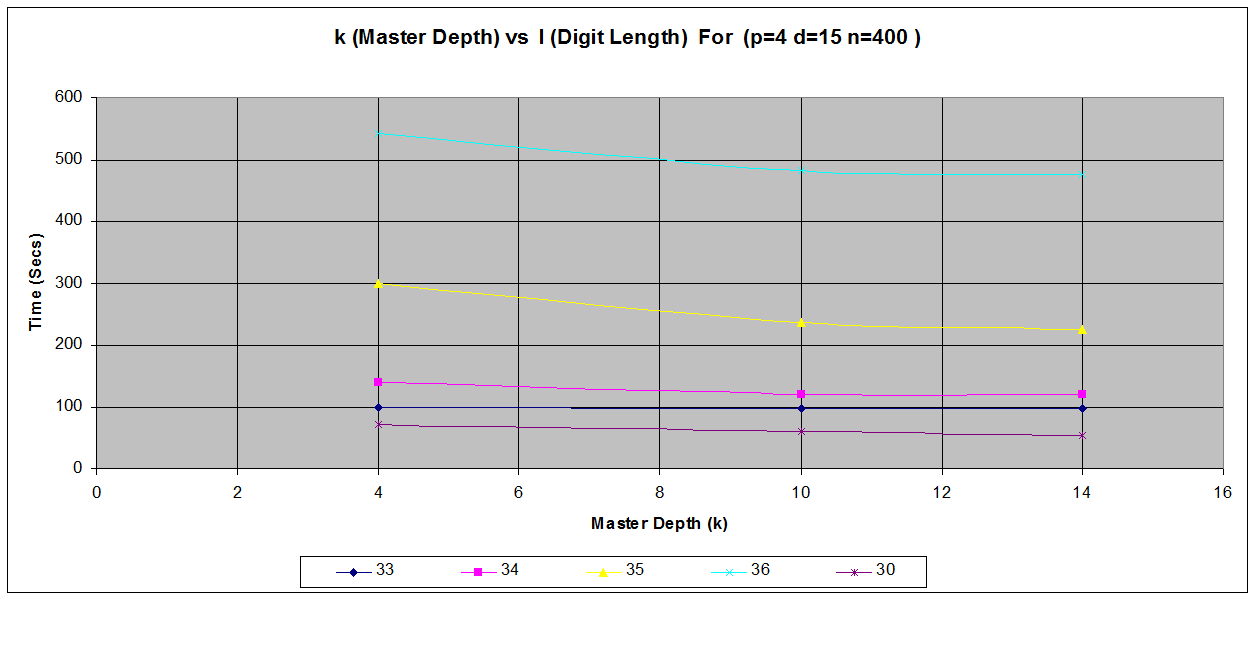
\includegraphics[scale=.46]{images/pdn_p=4-d=15-n=400} 
\caption{Runtime Vs K/L for p=4 d=15 n=400}
\label{Runtime Vs K/L for p=4 d=15 n=400}
\end{figure}

\begin{figure}[!htbp]
\centering
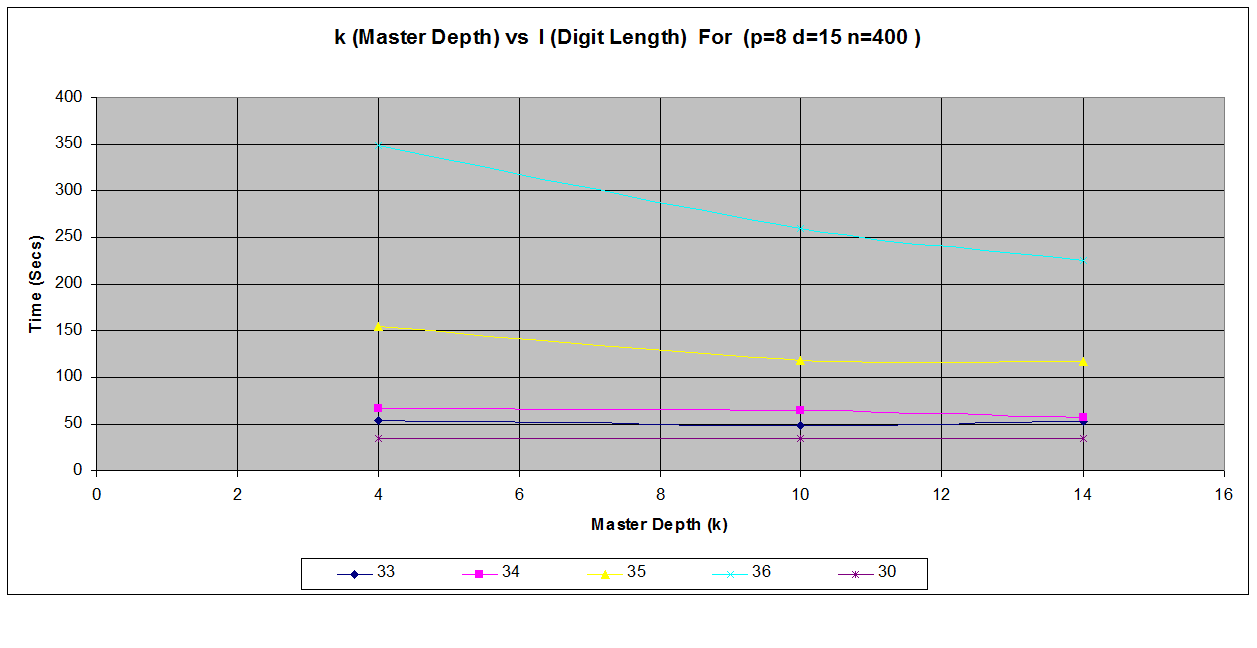
\includegraphics[scale=.46]{images/pdn_p=8-d=15-n=400} 
\caption{Runtime Vs K/L for p=8 d=15 n=400}
\label{Runtime Vs K/L for p=8 d=15 n=400}
\end{figure}

\begin{figure}[!htbp]
\centering
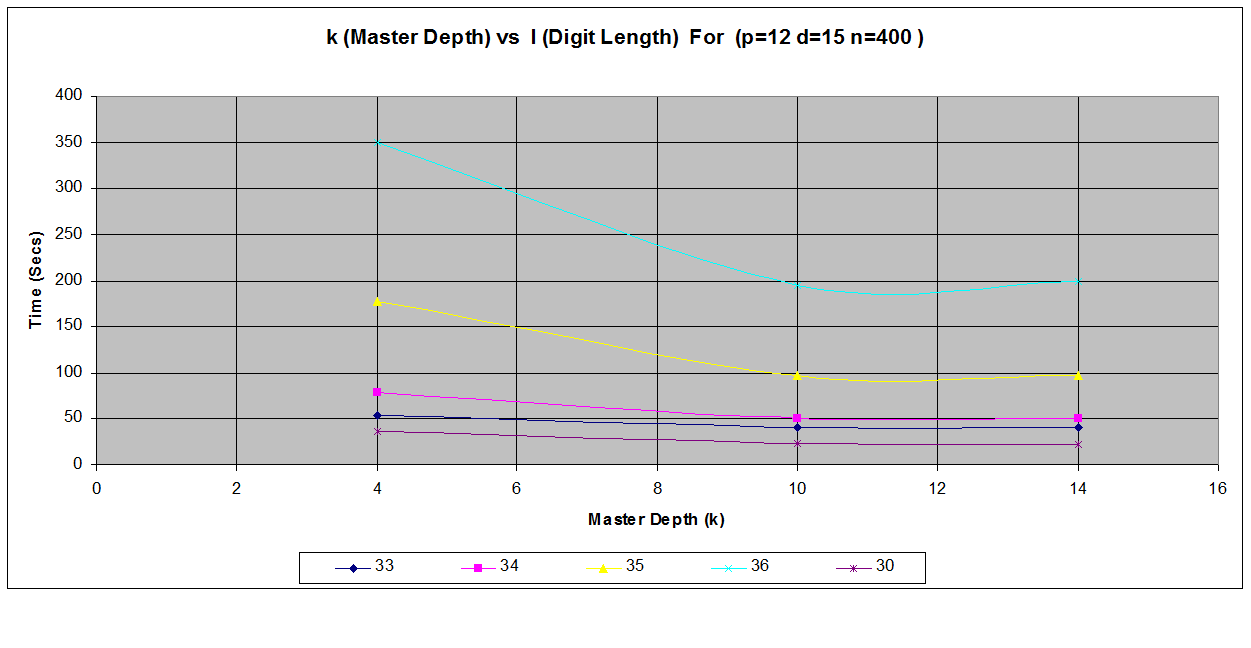
\includegraphics[scale=.46]{images/pdn_p=12-d=15-n=400} 
\caption{Runtime Vs K/L for p=12 d=15 n=400}
\label{Runtime Vs K/L for p=12 d=15 n=400}
\end{figure}

\begin{figure}[!htbp]
\centering
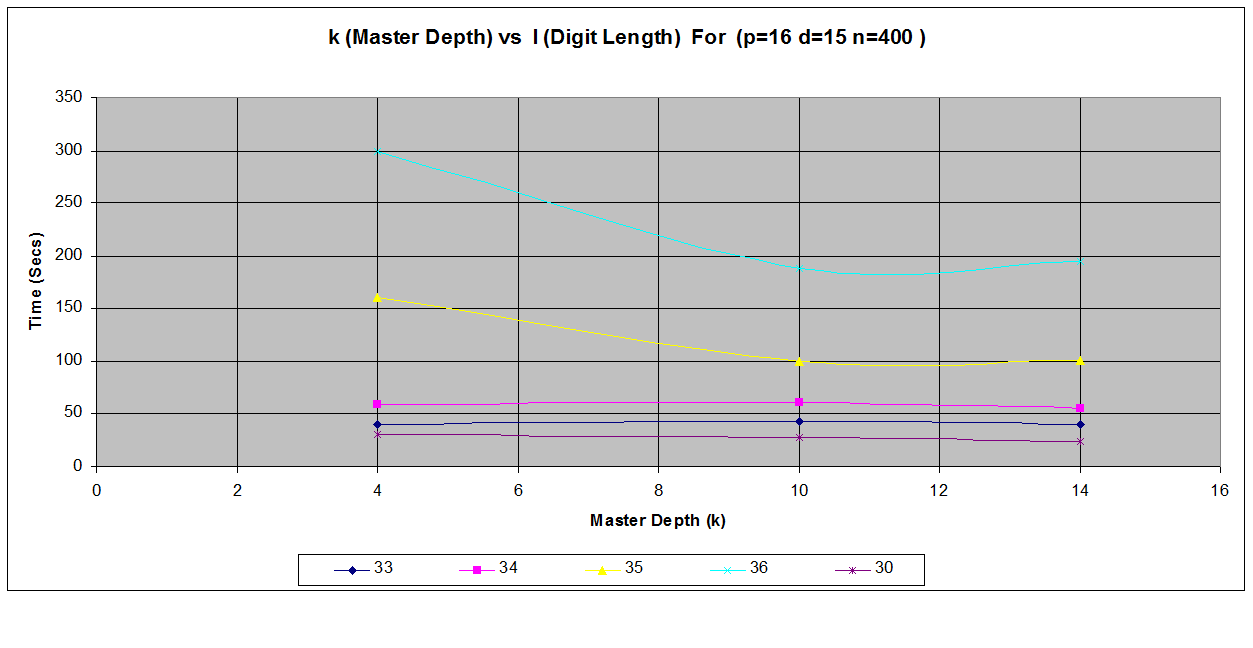
\includegraphics[scale=.46]{images/pdn_p=16-d=15-n=400} 
\caption{Runtime Vs K/L for p=16 d=15 n=400}
\label{Runtime Vs K/L for p=16 d=15 n=400}
\end{figure}

\begin{figure}[!htbp]
\centering
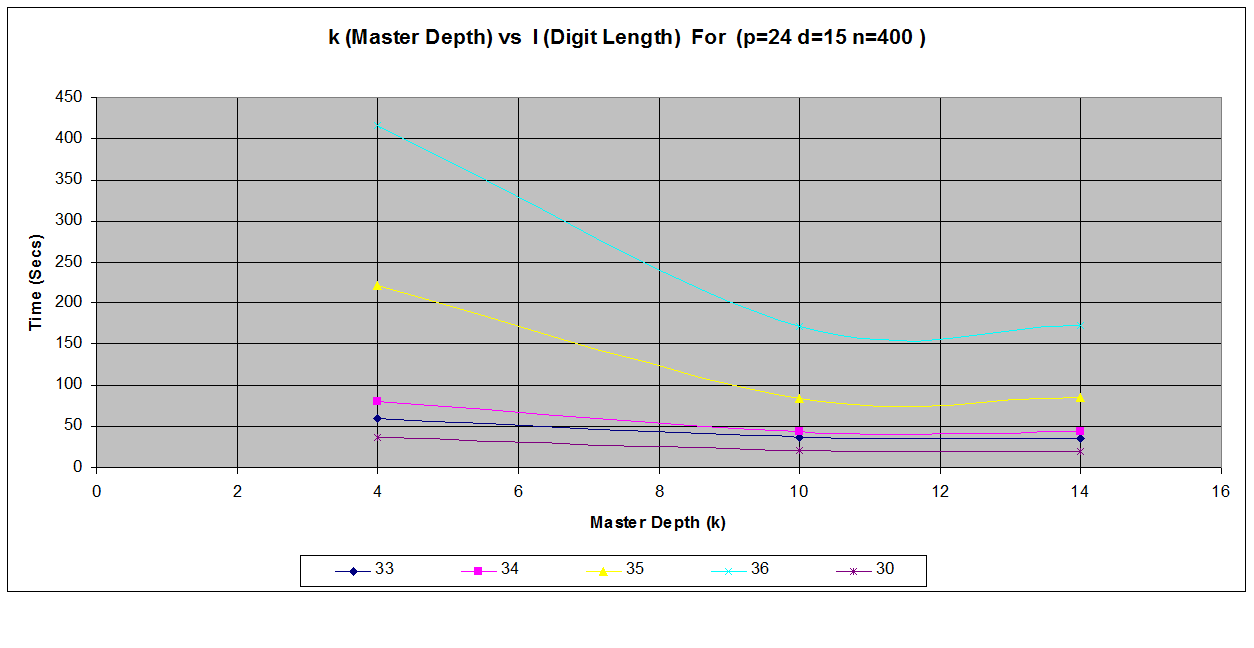
\includegraphics[scale=.46]{images/pdn_p=24-d=15-n=400} 
\caption{Runtime Vs K/L for p=24 d=15 n=400}
\label{Runtime Vs K/L for p=24 d=15 n=400}
\end{figure}



\pagebreak
\section{Conclusions}
\begin{itemize}
\item
The serial runtime of the algorithm is of the order of
\begin{align}
T(n,1) &= \sum_{c=0}^{d} 2^c *{l\choose c} * n\nonumber\\
&=\mathcal{O}( 2^d *{l\choose d} * n ) \label{p1_runtime_2}
\end{align}
This is borne out by the plots of the performance of the trial runs
\item
The plots show that the runTime of the algorithm appears to increase linearly with the number of problems $n$ as expected from the theoretical runtime in $\eqref{p1_runtime_2}$
\item
From the plots it can be seen that the runtime increases asymptotically with an increase in the integer length $l$, which is again as expected from the theoretical runtime from equation $\eqref{p1_runtime_2}$
\item
The parallel runtime for the algorithm with the correct value of  k in the range, $10<k<12$ and for number of processors $p=24$ is almost 6 times faster than the serial run time of the algorithm for the same size of the problem. For e.g for $l=36,n=400$ the serial algorithm has a runtime of $750$ seconds, the parallel algorithm with $p=24$, $k=11$ in comparison has a run time of $150$ seconds for the same problem size.
\item
The speedup of the parallel algorithm with the right $p$ and $k$ widens over the runtime of the serial algorithm as the size of the problem as defined by the Integer length $l$ increases.
\item
When a depth of $k$ is chosen, the worker processors will receive $\mathcal{O}(2^k)$ distributed evenly across them, so $k$ determines the optimum parallelism that can be achieved and needs to be carefully chosen
\item
While the runtime improves with the increase of parallel processors from $4$ to $24$, the best improvement in runtime is seen in the range of $k=10-12$ for the data considered in these runs
\item
There seems to be a inflexion point in $k$ in the range of $k=10-12$. From $k=4$ to this inflexion we can see a sharp improvement in runtime, further increase in $k$ beyond $12$ does not improve the performance. This effect of $k$ can be seen more pronounced as we move to higher values of $p$ from $p=4$ to $p=24$. 
\item
While parallelism with higher values of $p$ does give better performance for larger problems as defined by larger values of $l$ and $d$, just increasing the number of processors will not give the best increase in performance. It has to be ensured that the processors are optimally utilized for best efficiency and this has to be done by choosing the optimal value of $k$ at which work is best distributed between the processors and maximum efficiency and best speedup can be achieved. For the data considered in these runs it appears that a $k$ in the range of $10-12$ gives the best runtime, especially as the number of processors is increased to higher values.
\end{itemize}


% Generate the bibliography.
\bibliography{latex-sample}
\bibliographystyle{unsrt}

\end{document}


\end{document}